%Januar 2021 - März 2021


\documentclass[12pt]{article}

\usepackage{multicol}
\usepackage{geometry}
\usepackage{blindtext}
\usepackage{setspace}
\usepackage{hyperref}
\usepackage[headsepline=0.8pt, footsepline =0.8pt]{scrlayer-scrpage}
\usepackage{listings}
\usepackage{subcaption}
\usepackage{tabularx}
\usepackage{xurl} %Formats \url{}-entrys better
\usepackage{color, colortbl}
%\usepackage{pdfpages}
\usepackage{amssymb}
\usepackage{caption}
\usepackage{subcaption}
\usepackage{float}


\geometry{a4paper, top=25mm, left=35mm, right=25mm, bottom=25mm, headsep=13mm, footskip=12mm, head=14.5pt}

%encoding
%--------------------------------------
\usepackage[utf8]{inputenc}
\usepackage[T1]{fontenc}
%--------------------------------------

%German-specific commands
%--------------------------------------
\usepackage[ngerman]{babel}
%--------------------------------------

%Hyphenation rules
%--------------------------------------
\usepackage{hyphenat}
%--------------------------------------


\usepackage{graphicx}
\graphicspath{ bilder/}

\newcommand{\Autor}{Andreas Schmider}

\newcommand{\Bearbeitungszeitraum}{2 Semester}
\newcommand{\Kurs}{TINF19B3}
\newcommand{\Betreuer}{Prof. Dr.-Ing. Kai Becher}


% Images
\newcommand{\DHBWLogoDeckblatt}{\includegraphics[width=4.5cm]{Logos/dhbw-logo}}
\newcommand{\KernPackages}{\includegraphics[height=12cm]{Bilder/KernModul_Packages}}
\newcommand{\PluginPackages}{\includegraphics[height=7cm]{Bilder/PluginModul_Packages}}
\newcommand{\BridgePattern}{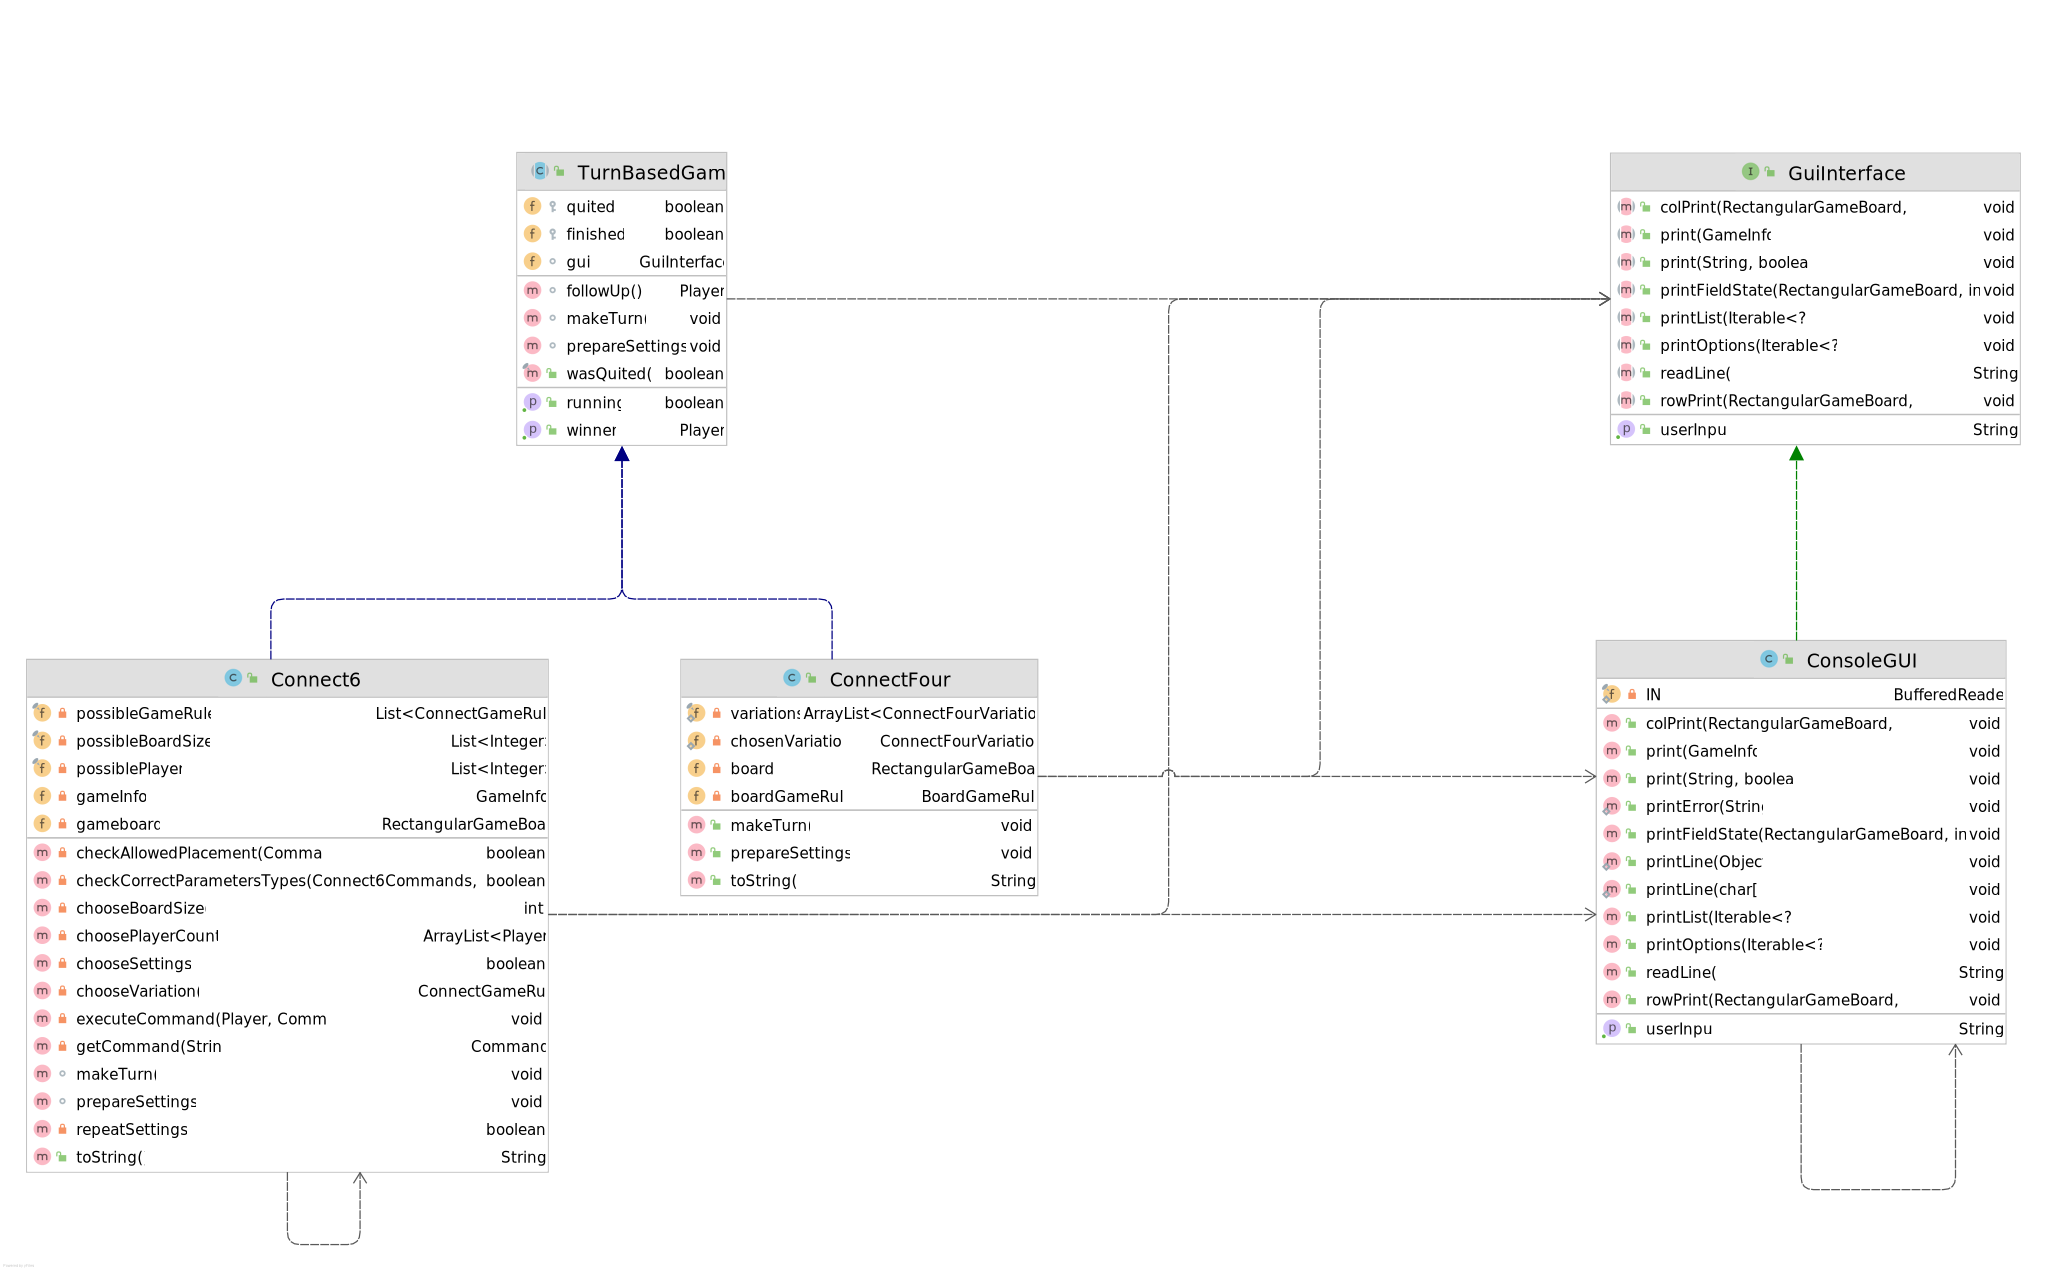
\includegraphics[height=7cm]{Bilder/Bridge_complete}}
\newcommand{\PrintList}{\includegraphics[width=15cm]{Bilder/printList}}
\newcommand{\RowPrint}{\includegraphics[width=15cm]{Bilder/rowPrint}}
\newcommand{\pkgGamerule}{\includegraphics[width=7cm]{Bilder/gamerules}}
\newcommand{\boardGR}{\includegraphics[width=15cm]{Bilder/BoardGameRule}}
\newcommand{\torus}{\includegraphics[width=15cm]{Bilder/Torus}}

\newcommand{\Titel}{Kleine Spielesammlung von 4-Gewinnt Versionen}
\newcommand{\ArtArbeit}{Studienarbeit}
\newcommand{\Abschluss}{Bachelor of Science}
\newcommand{\Studiengang}{Studiengang Informationstechnik}

\newcommand{\Ort}{Karlsruhe}

%\newcommand{\Abgabedatum}{16.02.2021}


\begin{document}
\onehalfspacing
\pagenumbering{Roman}
	\begin{titlepage}
		{\DHBWLogoDeckblatt}\\[2cm]
		\begin{center}
			\vspace*{-2cm}
			{\Huge \Titel}\\[2cm]
			{\Large \Abschluss}\\[0.5cm]
			{\large \Studiengang}\\[0.5cm]
			{\large an der}\\[0.5cm]
			{\large Dualen Hochschule Baden-Württemberg Karlsruhe}\\[0.5cm]
			{\large von}\\[0.5cm]
			{\large\bfseries \Autor}\\[1cm]
			{\large Abgabedatum 30. April 2022}
			\vfill
		\end{center}
		\begin{tabular}{l@{\hspace{1cm}}l}
			Bearbeitungszeitraum & \Bearbeitungszeitraum \\
			Kurs & \Kurs \\
		\end{tabular}
	\end{titlepage}

\newpage

\thispagestyle{empty}
\begin{center}
\Large\bfseries Erklärung
\end{center}
\medskip
\noindent
Wir versichern hiermit, dass wir unsere \ArtArbeit \ mit
dem Thema: 
\begin{center}
	 \Titel \ 
\end{center}
selbstständig verfasst und keine anderen als die angegebenen Quellen und
Hilfsmittel benutzt haben. Wir versichern zudem, dass die eingereichte elektronische Fassung mit der
gedruckten Fassung übereinstimmt.

\vspace{3cm}
\noindent
\underline{\Ort, 30. April 2022 \hspace{9cm}}\\
%\hfill\underline{\hspace{6cm}}\\
Ort, Datum\hfill Unterschrift\hspace{4cm}

\newpage

\thispagestyle{empty}
\setcounter{tocdepth}{2}
\tableofcontents

\newpage

%\thispagestyle{empty}
\thispagestyle{plain}
\cleardoublepage
\addcontentsline{toc}{section}{\listfigurename}
\listoffigures

\addcontentsline{toc}{section}{\listtablename}
\listoftables

\newpage


\thispagestyle{plain}
\pagenumbering{arabic}

\section{Beschreibung der Software}

\textbf{Beschreibung der Funktionalität}
\\
\noindent Aus einem alten Projekt existiert schon ein Connect6 Spiel, das in der Konsole gespielt wird. Dabei
gibt es einige Einstellungen die während des Programms noch gesetzt werden können. Somit kann
es von zwei bis vier Spielern gespielt oder die Spielfeldgröße auf 18x18 oder 20x20
festgelegt werden. Eine der größeren Auswirkung hat die Auswahl der Spielregeln.
Connect6 ist ähnlich wie Vier gewinnt und Ziel ist es mehrere Steine in eine Reihe zu legen.
Connect6 wird dabei aber auf einem Brett gespielt, das eben auf dem Boden liegt. So fallen die
Steine nicht bis in die letzte Zeile sondern bleiben an ihrem Platz. Ebenso werden pro Zug zwei
Steine pro Spieler gesetzt.
Bei der Standart-Spielregel zählen die Steine nur bis zum Spielfeldrand. Es gibt aber auch die
Torus-Version, bei dem die Steinreihen über den Rand hinaus gezählt werden. So beginnt das
Spielfeld erneut von oben, wenn man aus der untersten Zeile eins nach unten gehen würde.
\\

Zusätzlich dazu soll jetzt auch noch Vier Gewinnt mit unterschiedlichen Variationen/Regeln implementiert werden. Bei einer Variation soll es möglich sein, die Spielsteine nur von oben herunterfallen zu lassen. Bei einer anderen z.B. Drop Four ist es aber auch möglich den untersten Stein einer Spalte zu entfernen.
Bei dieser Spielesammlung soll es möglich sein mit wenig Aufwand neue Spielregeln/Variationen 
oder sogar ganz neue Spiele (die einen ähnlichen Aufbau haben) zu implementieren.
\\

Bei der Entwicklung dieser Software wurde zwar darauf geachtet einen möglichst strukturierten und einfachen Code zu erstellen,
es wurde sich aber nicht direkt an die in dieser Vorlesung besprochenen Themen gehalten. Es wurde zwar versucht die DRY-Regel anzuwenden, 
da diese mir schon selber in den Sinn gekommen ist, aber wie ich später festgestellt habe wurde diese nicht überall umgesetzt. Ebenso habe ich öfters kleinere Code Reviews vorgenommen und refactored, da mir immer wieder beim erneuten Anschauen aufgefallen ist, wie unverständlich der Code ist. Da der Code ursprünglich von einer Programmieraufgabe am KIT stammt, mussten auch Kommentare verwendet werden. Nachdem ich diesen Code aber nach über 3 Jahren wieder angeschaut habe ist mir klar geworden, dass trotz vieler Kommentare der Code sehr schwierig zu lesen ist.
\\ 

\noindent  \textbf{Beschreibung des Kundennutzens}
Der Kunde erhält Spaß und Unterhaltung.
\\

\noindent \textbf{Verwendete Technologien}
- Java
- JUnit 5
- IntelliJ
\\

\noindent \textbf{Link zum Repository}
\url{https://github.com/a-schmider/ASE_Substrat}

\newpage
\section{Unit tests}

\newpage
\section{Programming Principles}

\subsection{SOLID}

\subsubsection{Single-Responsibility-Principle}
Das Single-Responsibility-Principle soll dafür sorgen, dass jede Klasse nur eine Aufgabe erfüllt. Damit entstehen viele kleinere, unabhängigere Klassen. Sobald sich bei einer großen Klasse etwas ändert muss möglicherweise vieles auch in anderen Methoden angepasst werden. Wenn es viele kleine Klassen gibt, die nur für eine Sache zuständig sind, ist es nach der kleinen Änderung in einer Klasse getan und es müssen sonst nirgends Anpassungen gemacht werden (je nach Ausprägung der Änderung).
\\

Im Code wurde das zum Beispiel bei den Spielregeln angewendet. Für jede Spielversion gibt es eine Klasse die nur überprüft, ob ein Zug gemacht werden darf und ob ein Gewinner vorliegt. So gibt es bisher zwei Spielvarianten für Connect6 die in unterschiedlichen Klassen implementiert sind und nicht auf eine Helper-Klasse o.ä. angewiesen sind und dort die Spielvariante abfragen müssen um zu entscheiden ob ein Zug erlaubt ist oder nicht. Definiert wurde das über Interfaces und der abstrakten BoardGameRule-Klasse. Die davon abgeleiteten Klassen implementieren dafür weitere Methoden, die das besser strukturieren, aber keine, die zusätzliche , ungewollte Funktionen implementieren.

\begin{figure}[H]
\centering
{\boardGR}
\caption{Die abstrakte BoardGameRule-Klasse}
\label{fig:boardGR}
\end{figure}



\subsubsection{Open/Closed-Principle}
Programme sollten offen für Erweiterungen und geschlossen für Änderungen sein. So sollte im nachhinein keine Änderung mehr an bestehendem Code vorgenommen werden. Wenn die Software um Funktionen erweitert werden soll, soll das nur durch Erweiterung z.B. Unterklassen gemacht werden.
\\

Angewendet wurde das auf die Spielregeln. Zu Beginn gab es nur zwei Klassen für Spielregeln, die BoardGameRule- und die ConnectGameRule-Klassen. In ConnectGameRule wurde der grundsätzliche Ablauf für diese Art von Spielregeln erstellt. Durch die Unterklassen können aber neue Varianten implementiert werden, im Code mit den Connect6StandardGameRule- und Connect6TorusGameRule-Klassen. So könnten in Zukunft noch viele weitere Spielregel erstellt werden, welche diese Regeln anpassen ohne bestehenden Code zu ändern.

\begin{figure}[H]
\centering
{\torus}
\caption{Die Connect6TorusGameRule-Klasse}
\label{fig:torus}
\end{figure}



\subsubsection{Liskov-Substitution-Principle}
Dieses Prinzip wird eingehalten, wenn für jedes Oberklassenobjekt ein Unterklassenobjekt verwenden werden kann, ohne dass dies zu Fehlern oder unbeabsichtigten Verhalten führt. 
\\

Verletzt wurde dieses Prinzip bei den Spielbrettern. Es wurde nämlich ein quadratisches Spielfeld als Unterklasse eines Rechteckigen Spielfelds implementiert. Somit verhält sich das quadratische Spielfeld aber nicht nicht mehr wie ein Rechteckiges Spielfeld und schränkt die Funktionalität sogar ein, anstatt sie zu erweitern.
Es gibt zwar keine Methoden um die Länge und Breite zu setzen aber einen Konstruktor, der diese setzt. Dort könnte zwar ein Fehler geworfen werden aber das führt wieder zu \glqq schlechtem \grqq Code. Deshalb sollte dort ein neues Konstrukt angestrebt werden.



\subsubsection{Interface-Segregation-Principle}
Mit diesem Prinzip sollen, ähnlich wie beim Single-Responsibility-Principle, kleine kompakte Einheiten generiert werden. In diesem Fall aber mit Interfaces und nicht mit Klassen. So sollen Klassen immer alle Methoden etc. des Interfaces sinnvoll verwenden ohne diese nur zu implementieren, damit diese implementiert sind. Wenn es dazu kommt sollten lieber mehrere kleine Interfaces erstellt werden. Die Klasse müsste dann nicht mehr alle Interfaces implementieren, sondern nur noch die, die tatsächlich benötigt werden.
\\

Bisher gibt es in diesem Projekt nur drei Interfaces. Eins für die GUI und zwei für Spielregeln. Bei den Interfaces für Spielregeln gibt es das Winnable Interface, das die Methode checkWin(...) und das PlaceableCheck Interface, das eine checkAllowedPlacement(...) definiert. Bisher werden diese Zwei nur von der Klasse BoardGameRule verwendet. In Zukunft könnte es aber ein Spiel geben, z.B. Monopoly, bei dem es zwar einen Gewinner gibt, aber jeder Zug erlaubt ist sodass nur Winnable und nicht PlaceableCheck implementiert werden müsste.



\subsubsection{Dependency-Inversion-Principle}




\subsection{GRASP}
Im laufe der Vorlesung wurden neun Faktoren von General Responsibility Assignment Software Patterns/Principles (GRASP) besprochen. Davon wurden aber nur zwei (Low Coupling und High Cohesion) genauer besprochen und deshalb sollen in diesem Dokument auch nur diese beiden thematisiert werden.


\subsubsection{Low Coupling}
Um eine geringe Kopplung zu erhalten muss versucht werden die Klassen so unabhängig wie möglich voneinander zu machen. Dies kann zum Beispiel damit erreicht werden, dass keine spezielle Klasse sondern ein Interface als Parameter/Attribut verwendet wird. Dies kann auch mit Oberklassen gemacht werden, mit Interfaces sind die Klassen aber noch unabhängiger voneinander. Damit wird dann nur spezifiziert welche Methoden mit welchen Parametern unterstützt werden müssen. Wie genau die Klasse das dann umsetzt ist egal. So muss zu Beginn nicht gewusst werden welche Klassen genau verwendet werden. 
\\

Ein gutes Beispiel dafür ist das GuiInterface. Dieses besitzt eine Methode printList(Iterable<?>). Für diese Methode wird nur vorausgesetzt, dass eine Element übergeben werden muss über das iteriert werde kann. Es wäre auch möglich eine List<?> anstatt des Iterable<?> zu nehmen, da eine Liste auch das Iterable Interface implementiert und das in der Methode genutzt wird. Wenn aber eine Liste verwendet wird schränkt man die verwendbaren Klassen ein obwohl das gar nicht nötig wäre.
\\

\begin{figure}[H]
\centering
{\PrintList}
\caption{Die printList-Methoden Implementierung}
\label{fig:printList}
\end{figure}


Das GuiInterfaces enthält ebenfalls eine rowPrint(RectangularGameBoard)-Methode. RectangularGameBoard ist diesmal aber kein Interface sondern eine normale Klasse. Indem davon Unterklassen erstellt werden, wie Connect6GameBoard, können diese auch dafür verwendet werden. 
\\

\begin{figure}[H]
\centering
{\RowPrint}
\caption{Die rowPrint-Methoden Implementierung}
\label{fig:rowPrint}
\end{figure}

Die rowPrint Methode verwendet folgende drei Methoden der übergebende Klassen.
\begin{itemize}
\item getCountOfRows
\item getCountOfColumns
\item getFieldAsString
\end{itemize}

Es wäre auch möglich ein Interface zu erstellen, dass diese drei Methoden unterstützt. So wäre es nicht notwendig, dass das übergebende Objekt eine Unterklasse oder selber vom Typ RectangularGameBoard ist. Zum Beispiel könnten dann auch Tabellen unterstützt werden, die gar nichts mit Spielbrettern zu tun haben. Dies ist für diese Spielesammmlung aber nicht interessant, da nur Spielbretter verwendet werden. Somit könnte aber noch mehr Unabhängigkeit erzielt werden.



\newpage
\subsubsection{High Cohesion}
Um eine hohe Kohäsion zu erhalten, sollte versucht werden, Klassen oder Programmteile die zusammen arbeiten auch möglichst nahe beieinander zu halten z.B. in Packages oder Modulen. Ebenso sollte jede Klasse nur für eine Aufgabe zuständig sein siehe Single-Responsibility-Principle. Damit lässt sich schneller erkennen in welchem Bereich Änderungen vorgenommen werden müssen und welche andere Klassen davon betroffen sein könnten. Zu Kohäsion zählt aber auch wie gut die Daten und die Methoden einer Klasse zusammen passen und arbeiten.

So existiert in diesem Projekt ein Package (gamerules), dass für die Spielregeln verantwortlich ist. In diesem Package liegen die abstrakten Klassen und die Interfaces welche diese implementieren. Darin gibt es weitere Packages für die genauen Spielregeln der einzelnen Spiele (connect6 und connect\_four). So bald etwas an einem Interface oder der abstrakten Klassen geändert wird, erkennt man, dass alle anderen Klassen in diesem Package davon betroffen sein könnten.

\begin{figure}[H]
\centering
{\pkgGamerule}
\caption{Das gamerule-Package}
\label{fig:pkgGamerule}
\end{figure}



\subsection{DRY}
DRY steht für \glqq Don't repeat yourself \grqq. So soll möglichst kein Code mehrfach vorhanden sein und damit verhindern, dass der Quellcode unnötig groß und es möglicherweise zwei unterschiedliche Verfahren für die gleiche Sache verwendet wird. Natürlich können grundlegende Befehle nicht nur einmal verwendet werden aber es sollte darauf geachtet werden, das falls zwei Abschnitte eine ähnliche Funktion implementieren und nur minimale Unterschiede aufweisen, diese so anzupassen, dass die Unterschiede durch Parameter oder Verzweigungen generiert werden. Somit muss nur an genau einer Stelle etwas geändert werden und alle Funktionen die darauf aufbauen erhalten diese Änderung und müssen nicht manuell angepasst werden.
\\




\newpage
\section{Clean Architecture}
Dieses Programm wurde in zwei Schichten aufgeteilt. Dem Kern-Modul, in dem die ganzen Strukturen liegen, und dem Plugin-Modul, in dem momentan die Ausgabe/GUI realisiert wird. Um sicherzustellen, dass die Klassen im Kern die Plugins nicht kennen wurden Java Module verwendet und es wurde nur dem Plugin Modul gestattet die Klassen des Kerns zu verwenden und nicht andersherum. Dies ist wichtig, damit die Plugins ausgetauscht werden können ohne den Domain Code anpassen zu müssen.
\\

\begin{figure}[htpb!]
\centering
\begin{subfigure}{.5\textwidth}
  \centering
  {\KernPackages}\\[2cm]
  %\caption{A subfigure}
  \label{fig:sub1}
\end{subfigure}%
\begin{subfigure}{.5\textwidth}
  \centering
  {\PluginPackages}\\[2cm]
  %\caption{A subfigure}
  \label{fig:sub2}
\end{subfigure}
\caption{Kern- und Plugin-Module}
\label{fig:test}
\end{figure}





\newpage
\section{Entwurfsmuster evtl. Noch Template/Schablonen pattern}
Eines der Entwurfsmuster, das eingesetzt wurde ist das Brücken-Muster. Dies hat sich von selber eingeschlichen, als versucht wurde eine hohe Abstraktion zu erreichen. Genau dafür ist dieses Muster auch vorgesehen. Es soll die genaue Implementierung von der Abstraktion trennen. In diesem Fall wurde ein Interface erstellt, das die Benutzeroberfläche verwenden soll (GuiInterface). Dies ist der Implementierer in dem Design-Pattern. Bisher gibt es nur eine Klasse, die ConsoleGUI-Klasse, die dieses Interface implementiert und Ausgaben in der Konsole macht. Es sollte aber in Zukunft auch möglich sein eine weitere Klasse zu erstellen, die dann z.B. eine Graphische Benutzeroberfläche verwendet. Diese Klassen (ConsoleGUI und die folgenden) sind die Konkreten Implementierer des Interfaces. Aufgerufen werden die Implementierungen des GuiInterfaces von der TurnBasedGame-Klasse bzw. den Unterklassen, Connect6 und ConnectFour, da diese eine abstrakte Klasse ist. Dabei ist die TurnBasedGame-Klasse die Abstraktion und Connect6 und ConnectFour sind die speziellen Abstraktionen.

\begin{figure}[htpb!]
\centering
{\BridgePattern}\\[1cm]
\caption{Das Brücken-Entwurfsmuster}
\label{fig:bridge}
\end{figure}

Damit die Abstraktionen das Interface verwendet können, besitzen sie dieses als Attribut. In TurnBasedGame wird dieses jedoch noch nicht instanziiert, da es dort nicht verwendet wird. Erst in den Unterklassen werden diese in dem Konstruktor instanziiert. Erst damit ist es möglich die Methoden des Interfaces zu verwenden.

\newpage
\section{Refactoring}


\end{document}